\chapter{Discrete Events Systems}

As we introduce a definition of system and define hypothesis about it, we can now focus on a separated part of sequential system : the Discrete Event Systems also named DES. They have been introduced by B.ZEIGLER and have been evolving ever since.


\section{Definition of Discrete Event systems}

Discrete Event Systems (DES) are dynamic systems evolving at the rate of a series of discrete events. Discrete events are events that can possibly be physical or numerical, and they are over varying intervals, sometimes unknown \cite{controlOfDiscreteEvent_Ramadge}. These physical events are associated with occurrences in our system, and they will be developed later in this chapter.

Therefore, DES depend on a set of \emph{state variables}. We will take the previous vector to adapt it to the DES. In this new case, the \emph{state variable} $x$ is the set of states attainable by the system. We note this :
\begin{equation*}
x \in \cal{Q} \text{ with $\cal{Q}$  ensemble of attainable states}
\end{equation*}

Attainable states are most of time an infinite number, especially if the assumptions posed in \ref{ModelingSystem} are respected.

 %etry or input ?  / Inputs (j'ai corrigé un peu le sens pour faire apparaitre l'enseble des évenements Sigma plus loin en citant SAMPATH ) -Lucien
The inputs of the system that was previously $u$ rated will now belong to the events set. The dynamics of the system no longer depend upon a time, but on all possible events. Thanks to that new informations, we obtain a mathematical relationship that we will simplify by the following formula :
\begin{eqnarray}\label{stateSpaceDES}
\left\lbrace
\begin{aligned}
x_s &= f(x, u)\\
y  &= g(X, u) 
\end{aligned}
\right.
\end{eqnarray}
the two functions $f$ and $g$ being linear, non deterministic and invariant. The dynamic system is controlled by $f$ : it uses event on $u$ and the present state $x$ in order to evaluate the new system state $x_s$.

If for each inputs, we linked it with an event, we allowed to obtain a set of events rated $\Sigma$. We could find, for example, a formulation of DES which is well known and which could be used to study the diagnosability of a system \cite{DiagnostabilityOfDES}: 
\begin{align}\label{ModelSystemSampath}
G = (x, \Sigma, \delta, x_0)
\end{align}
The $f$ function presented in \ref{stateSpaceDES} is now represented by $\delta$, the transition function. Then, we have $x_0$ is the initial state, $\Sigma$ is the set of events and $x$ the actual state. 

% In the case of the labyrinth, events with discrete events make it possible to model the dynamics of displacement of the different objects. These movements are controlled by commands, sudden, manual or automatic. 
% \begin{equation*}
% u \in \cal{E} \text{ with $\cal{E}$ ensemble of event possible} 
% \end{equation*}

% Some state are generating different output as seen in previous section,\ref{System}. These outputs are include in a ensemble of output noted $\cal{S}$. 

% The evolution of a DES is always responding to this condition :\begin{align}\label{evolutionDES}
% \left\lbrace
% \begin{aligned}
% &X(k+1) = f(X(k), u)\\
% &S = g(X(k), u)
% \end{aligned}
% \right.
% \end{align}
% where $k \in \mathbb{N}$ is the incrementation of time. Therefore, it exist, for $k=0$, an initial state : $X(0) = X_0$. With the previous system definition, we also can evaluate, that for $k\in \mathbb{N}$, we have $X \in \cal{Q}$, an infinite numbers of state is possible.

\section{DES and finite state}
A part of DES exists with a specific state vector : it is not a vector and can only take one value. We called it a finite state Discrete Event System because : \begin{align*}
x\in \cal{Q} \text{ where $Q$ is only between [0,n]}
\end{align*}


 %%%%%%%%%%% ERREUR SCIENTIFIQUE  %% Oui j'avoue, c'est un peu nul... -Lucien
%Therefore, we can represent DES model with a graph but it's not the point that we would introduce because it's referring to graph theory but 

These DES admit another theory that we would like to introduce right now : the theory of automatons and languages. This finite state DES is a logical model as presented by Ramadge and Murray Wonham \cite{controlOfDiscreteEvent_Ramadge}, and it is possible to list the occurrences of events in this type of system. 
	
%A modifier
%This trajectory of the system is a prelude to the language accepted by the system. therefore, the theory of automatons which will be presented below. 

In the following sections, we will introduce our labyrinth problem in the DES concept then, we will study more precisely the theory just such introducing in this chapter.


\section{Introduction of DES in labyrinth}

In order to introduce DES in our dynamic labyrinth, we join each movement of object or wall as an event. So we have a list of elements : 
%scattered : balancé partout :D
\begin{align*}
\Sigma = \lbrace H, B, G, D, W_d, W_r \rbrace
\end{align*}
with each event equivalent to :
\newline 
\begin{minipage}{.5\textwidth}
\begin{itemize}
\item $H$ for up movement
\item $B$ for down movement
\item $G$ for left movement
\item $D$ for right movement
\end{itemize}
\end{minipage}
\begin{minipage}{.5\textwidth}
\begin{itemize}
\item $W_d$ for wall down movement
\item $W_r$ for wall right movement
\end{itemize}
\end{minipage}
\newline

Here is a quick representation of a possible sequence of a labyrinth in 2D, to this 9 possible cells labyrinth. Each movement of an object is subject to the system dynamics indicating it can only move from cell to cell.
\begin{figure}[H]
\begin{minipage}{0.5 \textwidth}	
      \begin{center}
      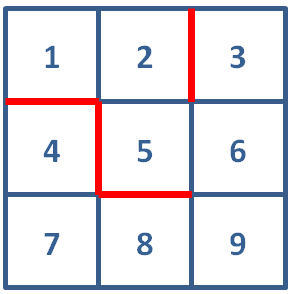
\includegraphics[height = 4cm]{./III/3x3lab.png}
%      \caption{Example - Labyrinth}\label{DES_labyrinth} % ligne originale
       \caption{\label{DES_labyrinth}Example - Labyrinth} % Correction david
      \end{center}
\end{minipage}
\begin{minipage}{0.5 \textwidth}
\begin{center}
      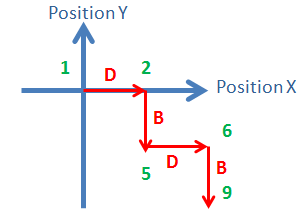
\includegraphics[height = 4cm]{./III/3x3graphe.png}
      \caption{\label{DES_labyrinth_sequence}Example - Graph of path}
      \end{center}
\end{minipage}
\end{figure}

%ERREUR FIGURE
The sequence represented here starts in the state modeled on the figure \ref{DES_labyrinth}, object starts in position $1$. The sequence going from 1 to 9 is the one shown in \ref{DES_labyrinth_sequence} : $D \rightarrow B \rightarrow D \rightarrow B$. 

%A reecrire
In the next part, we will explain the tools of automatons theory that we will use for the continuation of the project to analyze his kind of sequence and we will define a strong formalism we are going to use.

